\documentclass{article}

\usepackage[a4paper]{geometry}
\usepackage[ngerman]{babel}
\usepackage[utf8]{inputenc}
\usepackage[T1]{fontenc}
\usepackage{tabularx}
\usepackage{hyperref}
\usepackage{graphicx}

\graphicspath{{./diagrams/}}

\hypersetup{colorlinks=true, linkcolor=black, filecolor=black, urlcolor=black}

\begin{document}

\begin{titlepage}
	\begin{flushleft}
		TH Brandenburg \\
		Online Studiengang Medieninformatik \\
		Fachbereich Informatik und Medien \\
		Softwaretechnik \\
		Prof. Dr-Ing. Martin Schafföner
	\end{flushleft}

	\vfill

	\begin{center}
		\Large{Einsendeaufgabe 2: UML}\\[0.5em]
		\large{Sommersemester 2021}\\[0.25em]
		\large{Abgabetermin 02.06.2021}
	\end{center}

	\vfill

	\begin{flushright}
		Maximilian Schulke \\
		Matrikel-Nr. 20215853
	\end{flushright}
\end{titlepage}

\tableofcontents

\newpage

\section{Aufgabenstellung}

Im Moodle-Kurs wurde folgende Aufgabenstellung bekannt gegeben:

\begin{quote}
	Die Aufgabenstellung benötigt Ihre bisherigen Ergebnisse aus der ESA1.
	Bitte entwerfen Sie für Ihre in ESA1 entworfene Problemstellung zwei
	verschiedene UML-Diagramme, die sich jeweils an verschiede
	Interessenvertreter bzw. Projektteilnehmer richten sollen. Die Lösung MUSS
	ein Klassendiagramm und ein Aktivitätsdiagramm enthalten. Begründen Sie,
	welches weitere UML-Diagramm sie als nächstes erstellen würden. Beim
	Klassendiagramm können Sie auf die detaillierte Darstellung von Methoden
	verzichten, wichtige Attribute sollen jedoch enthalten sein. Achten Sie auf
	richtige Verwendung von Assoziation, Aggregation und Komposition sowie auf
	Multiplizitäten.
\end{quote}

\newpage

\section{Klassendiagramm}

\vfill

Für Entwicklungsteam

\begin{figure}[h]
	\centering
	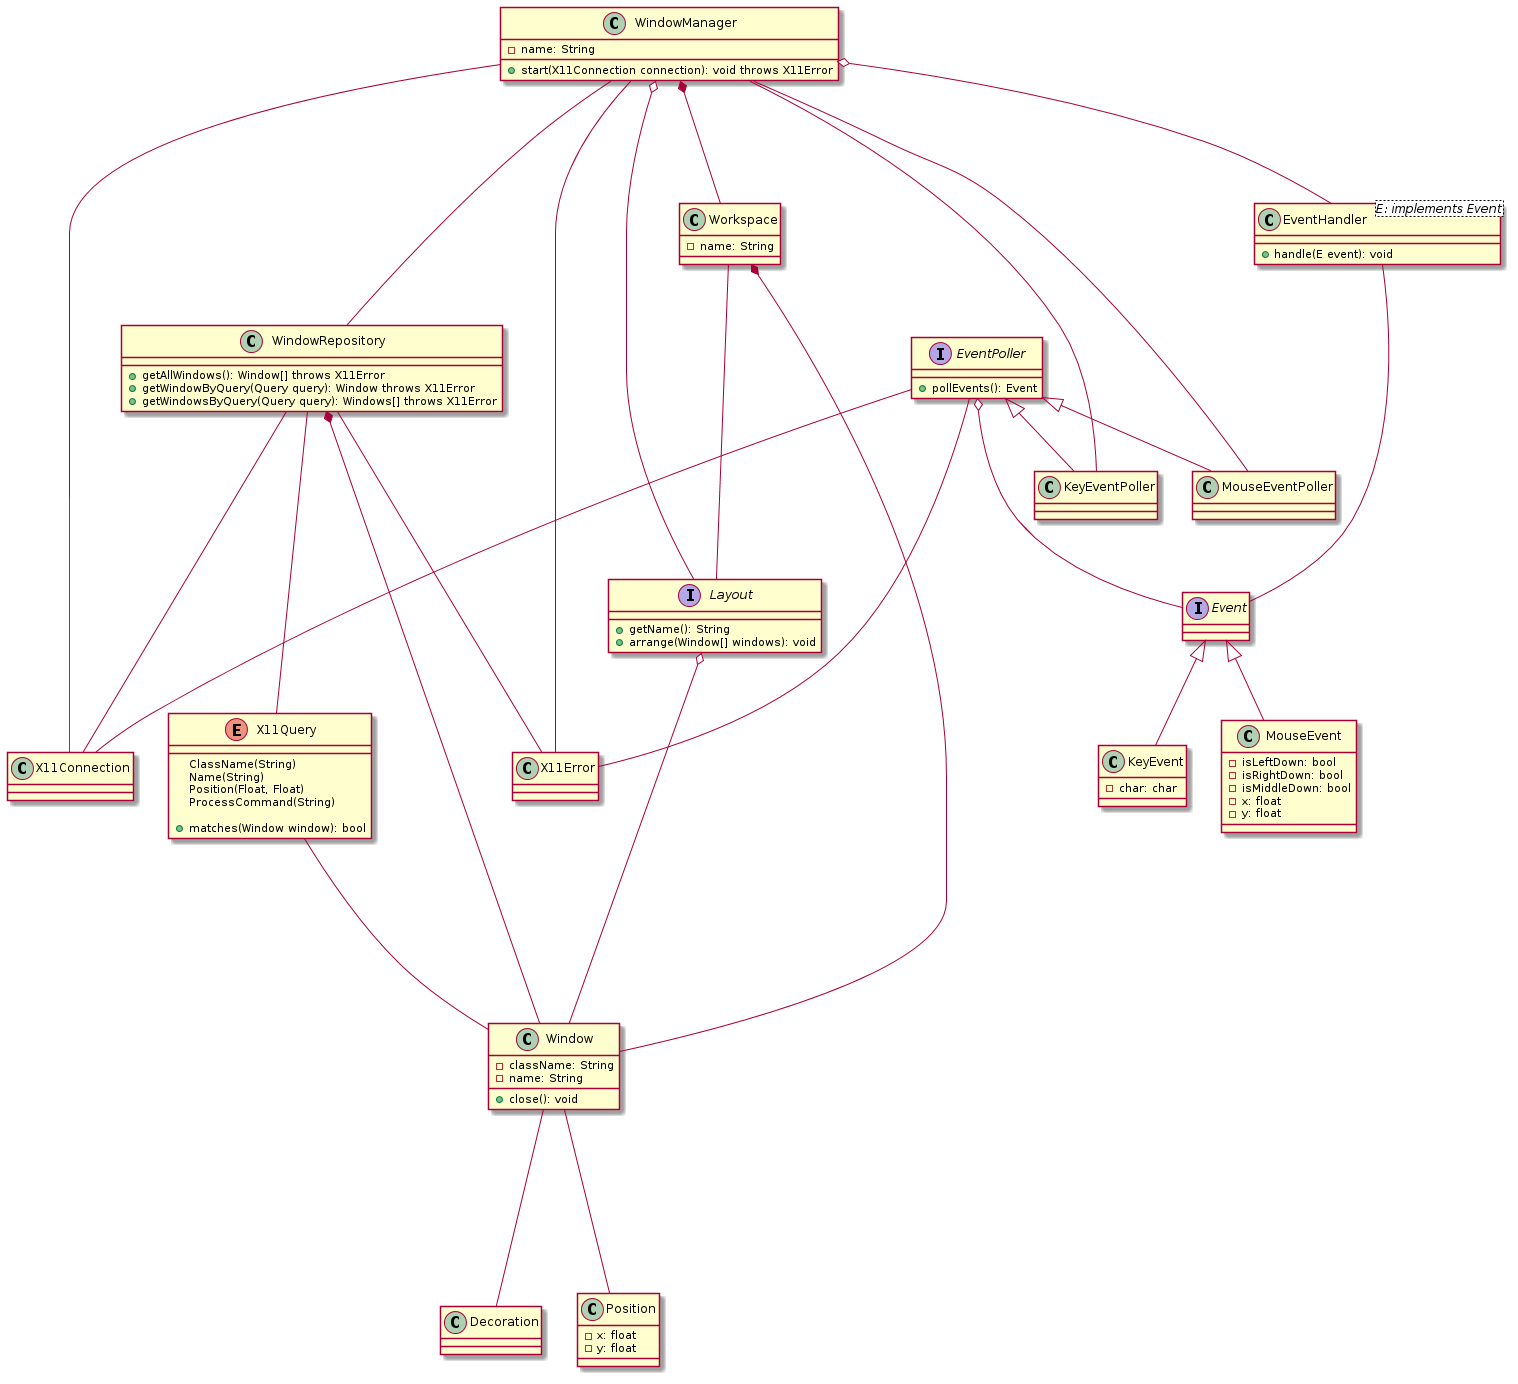
\includegraphics[width=\textwidth]{class}
	\caption{Klassendiagramm}
\end{figure}

\vfill

\newpage

\section{Aktivitätsdiagramm}

\vfill

Evtl Aktivitätsdiagramm = Benutzer "Konfigurierender"

\begin{figure}[h]
	\centering
	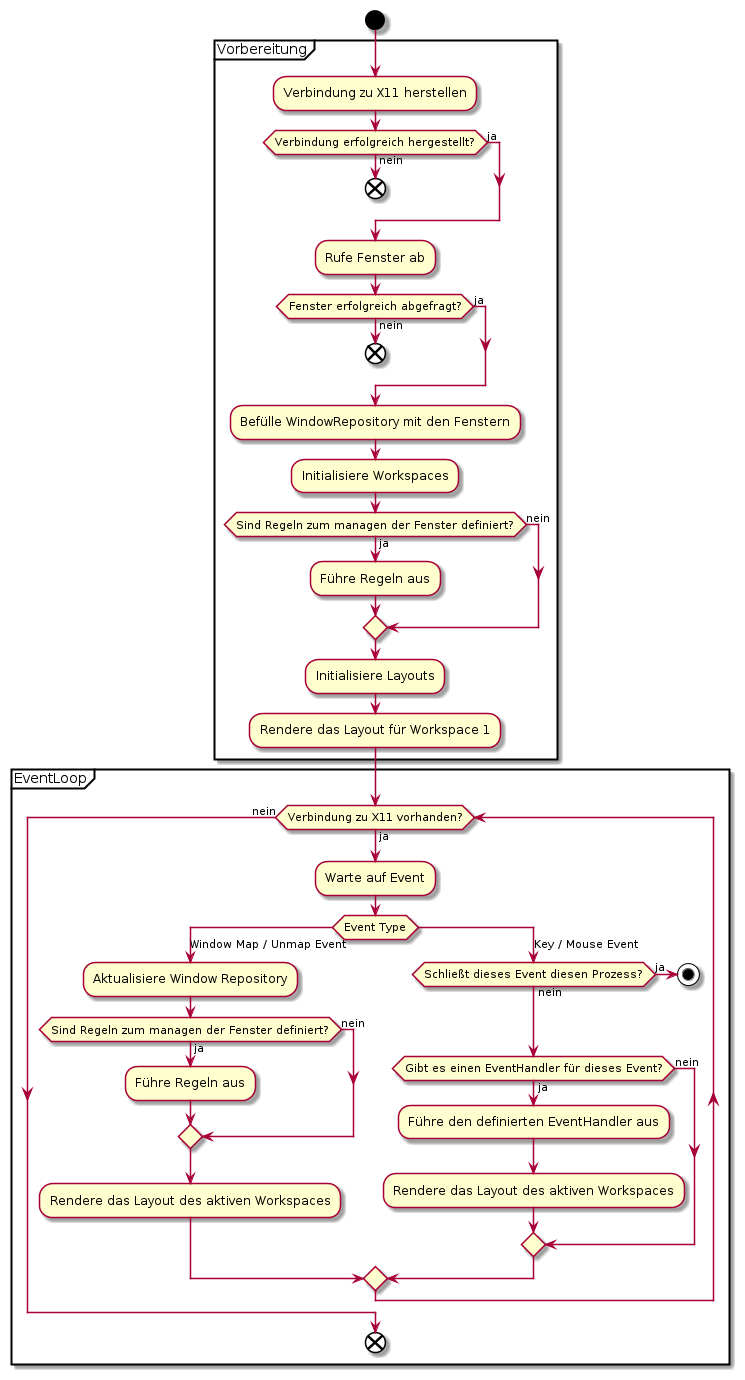
\includegraphics[height=0.725\textheight]{activity}
	\caption{Aktivitätsdiagramm}
\end{figure}

\vfill

\newpage

\section{Empfehlung für ein weiteres Diagramm}

\end{document}
